
% ? The state-of-the-art should show the reader a broad overview of techniques available and how they are related to one another in a hierarchical way like a mindmap. Describe the methods briefly and explain the weaknesses and strengths of the methods and how you want to use them to solve your problem.

\section{Motivation and State of the Art}

Representative datasets for Text-to-SQL include the WikiSQL \cite{zhong_seq2sql_2017} dataset and the SPIDER \cite{yu_spider_2019} dataset, which contains more complex SQL queries.
% We will also take a shallow look at older datasets and why they are not in use anymore in Text-to-SQL studies.
The former case consists of Single Table - Multiple Question and the latter case Multiple Table - Multiple Question. The top models available for Text-To-SQL will be studied, and the implementation of a couple of currently best methods will be reviewed and discussed in this study.

In this thesis, we will review the Text-to-SQL Challenges and datasets and structure of existing datasets and difference between them. Datasets to be covered are: ATIS, GeoQuery, IMDb, Advising, WikiSQL, Spider.

\subsection*{Datasets}

\subsubsection*{ATIS (Air Travel Information System) Dataset}

A relational schema is used to organize data from the official airline guide in the ATIS corpus. There are 25 tables containing information about fares, airlines, flights, cities, airports, and ground services. All questions related to this dataset can be answered using a single relational query. The relational database uses shorter tables for this dataset to answer queries intuitively.


Here is an example query from the ATIS dataset: Input is in natural language, and the output is in \lambda calculus.

\begin{figure}[htb]
    \centering
    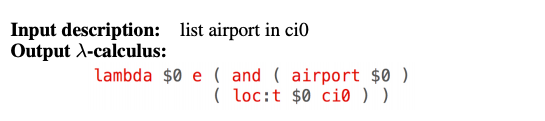
\includegraphics[width=0.8\textwidth]{pics/db/ATIS.png}
    \caption{Example from ATIS dataset for semantic parsing}
    \label{fig:ATIS}
\end{figure}

\subsubsection*{GeoQuery Dataset}

United States geography is represented in the Geoquery dataset. About 800 facts are expressed in Prolog. State, city, river, and mountain information can be found in the database. Geographic and topographical attributes such as capitals and populations make up the majority of the attributes.

\subsubsection*{IMDb Dataset}

The IMDb dataset contains 50K reviews from IMDb. There is a limit of 30 reviews per movie. Positive and negative reviews are equally represented in the dataset. The dataset creators considered a negative review with a score of 4 out of 10 and a positive review with a score of 7 out of 10. When creating the dataset, neural reviews are not taken into account. Furthermore, Training and testing datasets are equally divided.

\begin{figure}[htb]
    \centering
    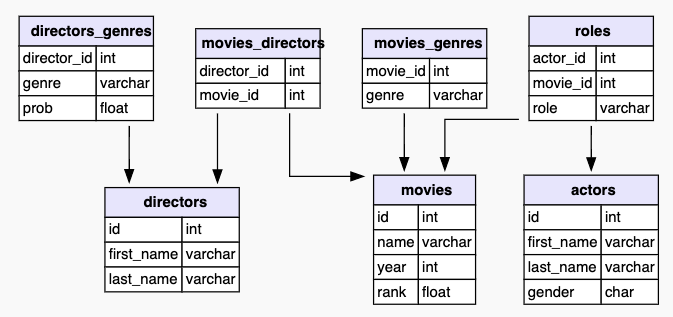
\includegraphics[width=0.8\textwidth]{pics/db/IMDb.png}
    \caption{Database Structure of IMDb dataset}
    \label{fig:IMDb}
\end{figure}

\subsubsection*{Advising Dataset}

The Advising dataset was created in order to propose improvements in text2SQL systems. The creators of the dataset compare human-generated and automatically generated questions, citing properties of queries that relate to real-world applications. Dataset consists of questions from university students about courses that lead to particularly complex queries. The database contains fictional student records. The dataset includes student profile information, such as recommended courses, grades, and previous courses. In an academic advising meeting, students were asked to formulate questions they would ask if they knew the database. Many of the queries in this dataset were the same as those in ATIS, GeoQuery, and Scholar.

% Figure 4:Example from Advising Dataset (Source: [1])
% pics/db/Advising.png
\begin{figure}[htb]
    \centering
    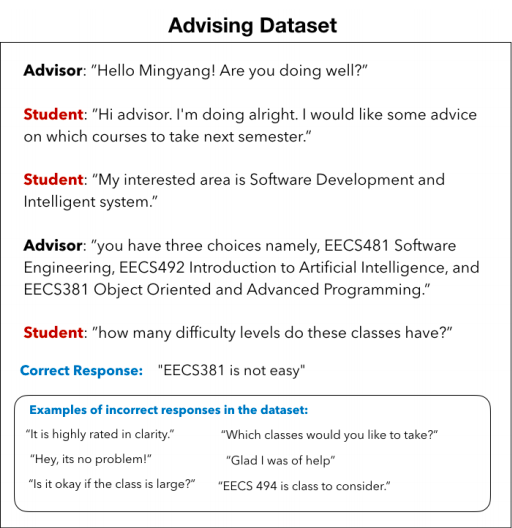
\includegraphics[width=0.8\textwidth]{pics/db/Advising.png}
    \caption{Example from Advising dataset}
    \label{fig:Advising}
\end{figure}

\subsubsection*{WikiSQL Dataset}

WikiSQL consists of 80K+ natural language questions and corresponding SQL queries on 24K+ tables extracted from Wikipedia. Neither the train nor development sets contain the database in the test set. Databases and SQL queries have simplified the dataset's creators' assumptions. This dataset consists only of SQL labels covering a single SELECT column and aggregation and WHERE conditions. Furthermore, all the databases contain only one table.

The database does not include complex queries involving advanced operations like JOIN, GROUP BY, ORDER BY, etc. Prior to the release of SPIDER, this dataset was considered to be a benchmark dataset. Using WikiSQL has been the subject of a great deal of research. WikiSQL's "WHERE" clause has been recognized as one of the most challenging clauses to parse semantically, and SQLNet and SyntaxSQL were previous state-of-the-art models.


% Figure 6: Example from WikiSQL dataset (Source: [6])
% pics/db/WikiSQL.png
\begin{figure}[htb]
    \centering
    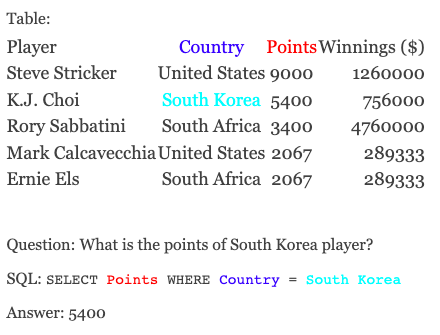
\includegraphics[width=0.8\textwidth]{pics/db/WikiSQL.png}
    \caption{Example from WikiSQL dataset}
    \label{fig:WikiSQL}
\end{figure}

\subsubsection*{Spider Dataset}

Yale University students created this dataset.
The SPIDER database contains 10K questions and 5K+ complex SQL queries covering 138 different domains across 200 databases. As opposed to previous datasets (most of which used only one database), this one incorporates multiple datasets. Creating this corpus was primarily motivated by the desire to tackle complex queries and generalize across databases without requiring multiple interactions.

% Figure 7: The annotation process of our Spider corpus (Source: [5])
% pics/db/Spider.png

\begin{figure}[htb]
    \centering
    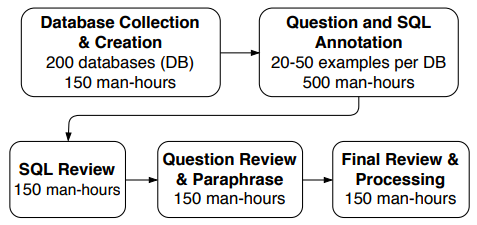
\includegraphics[width=0.8\textwidth]{pics/db/Spider.png}
    \caption{Example from Spider dataset}
    \label{fig:Spider}
\end{figure}

Creating a dataset involves three main aspects: SQL pattern coverage, SQL consistency, and question clarity. Several databases from WikiSQL are included in the dataset. The table is complex as it links several tables with foreign keys. In SPIDER, SQL queries include: SELECT with multiple columns and aggregations, WHERE, GROUP BY, HAVING, ORDER BY, LIMIT, JOIN, INTERSECT, EXCEPT, UNION, NOT IN, OR, AND, EXISTS, LIKE.

% Example 8: Example of Question-Query set from SPIDER (Source: [5])
% pics/db/Spider2.png
\begin{figure}[htb]
    \centering
    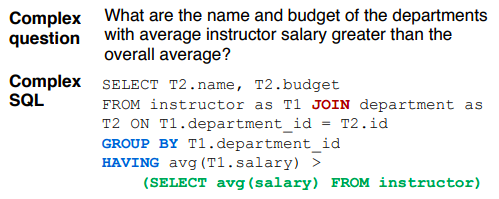
\includegraphics[width=0.8\textwidth]{pics/db/Spider2.png}
    \caption{Example of Question-Query set from SPIDER}
    \label{fig:Spider2}
\end{figure}

SPIDER's exact matching accuracy was 12.4\% compared to existing state-of-the-art models. As a result of its low accuracy, SPIDER presents a strong research challenge. Current SPIDER accuracy is around 66\% with an exact set match without values (refers to values in the WHERE clause) and around 63\% with values.

\subsection*{Models}

% Furthermore, Text-to-SQL models and techniques represented in the SPIDER challenge will be studied and evaluated. 
The research section will assess the best state-of-the-art research in this field, the T5\cite{raffel_exploring_2020} Transformer with PICARD\cite{scholak_picard_2021} (2021), RAT-SQL\cite{wang_rat-sql_2021} (2019), BRIDGE v1 and v2\cite{lin_bridging_2020} with BERT, HydraNet\cite{lyu_hybrid_2020} (2020), some novel methods in recent years, and some older models like Seq2SQL\cite{zhong_seq2sql_2017} (2017) and SQLova\cite{hwang_comprehensive_2019} (2019).

\begin{itemize}
    \item Seq2SQL and SQLNet will perform encoding using LSTM/Bi-LSTM and decode using classification and Pointer Network.
    \item SQLova and HydraNet encode natural language queries through a language model and decode them through the Natural Language-to-SQL layer, converting them to SQL grammars. Going a little further, SQLova was the first to use a language model as an encoder, encode questions and columns, and then predict queries.
    \item HydraNet uses BERT's token to rank columns one by one to fill in the slots of the SQL Query statement. Brief description of the BERT will be given in our final report.
    \item Since the SPIDER dataset used for RAT-SQL and BRIDGE is a Multi-Table, it is necessary to understand the Schema's relationship to the question and its internal relationships, for which Schema Linking and Encoding are applied, and decoders such as SemQL are utilized.
    \item RAT SQL reflects the schema information into the encoding and decoding with SemQL, including the relationships extracted from the question-scheme contextualized graph in Self-Attention.
    \item BRIDGE achieves Schema Linking by including the Schema's Table and Column Name and Value in the Encoding and utilizes the Pointer Generator Network as the Decoder.
          \newpage
    \item PICARD proposes a new method for simple and effective constrained decoding with large pre-trained language models.
          On both the SPIDER cross-domain and cross-database Text-to-SQL dataset and the CoSQL SQL-grounded dialog state tracking dataset, we find that the PICARD decoding method not only significantly improves the performance of fine-tuned unmodified T5 models but it also lifts a T5-3B model to state-of-the-art results on the established exact-match and execution accuracy metrics.
\end{itemize}

After reviewing research papers of these models, we will study implementation steps of these models. And at last, we will use our private dataset to evaluate the accuracy of each models for our data and if they are usable and reliable enough for our usage.

Most of these studies have excellent documentation regarding their implantation. Execution of these studies will be documented and published on Github. Nonetheless, In case of old and impractical implementation instructions, we will skip the implementation and continue with the top models available.


% [1] Vig, Jesse, and Kalai Ramea. “Comparison of transfer-learning approaches for response selection in multi-turn conversations.” Workshop on DSTC7. 2019.

% [2] Maas, Andrew, et al. “Learning word vectors for sentiment analysis.” Proceedings of the 49th annual meeting of the association for computational linguistics: Human language technologies. 2011.

% [3] Sun, Zeyu, et al. “A grammar-based structural CNN decoder for code generation.” Proceedings of the AAAI Conference on Artificial Intelligence. Vol. 33. 2019.

% [4] Finegan-Dollak, Catherine, et al. “Improving text-to-SQL evaluation methodology.” arXiv preprint arXiv:1806.09029 (2018).

% [5] Yu, Tao, et al. “Spider: A large-scale human-labeled dataset for complex and cross-domain semantic parsing and text-to-SQL task.” arXiv preprint arXiv:1809.08887 (2018).

% [6] Hwang, Wonseok, et al. “A comprehensive exploration on wikisql with table-aware word contextualization.” arXiv preprint arXiv:1902.01069 (2019).

